
Uno de los puntos centrales de este trabajo es exponer el estado del arte en el uso de Golang.
En concreto su uso para el desarrollo de software que enfrente problemas de tiempo real y interacción con hardware para control automático de actuadores.
En dicho estudio se ha consultado distintas publicaciones.
Citaremos varios estudios que resumen el nicho de Go como lenguaje de programación.

Los recursos consumidos por el lenguaje es uno de los primeros puntos que se deben evaluar.
Cual es el coste de hardware para ejecutar el código.

El rendimiento en la interacción del lenguaje con la base de datos, en concreto mysql por ser la más extendida, es uno de los primeros puntos que se han consultado.
En una comparación con Node.js, un framework muy extendido de javascript, la conclusión que extrae el estudio~\cite{Effendy20211955} es que: “\ldots la combinación de Go y MySQL es superior en el uso de CPU y utilización de memoria mientras que Node.js y MySQL es superior en tiempo de respuesta“.
No es inferior ni superior de forma relevante.

El rendimiento de utilización de RAM y CPU a la hora de enfrentar problema de algorítmica intensiva es el siguiente punto consultado.
En algorítmica con altos requerimientos, en particular la implementación de un árbol de decisiones~\cite{Dymora20201} la conclusión que extraen es que golang no presenta ventajas, tampoco inconvenientes, en materia de tiempos de ejecución.
Teniendo peor rendimiento en uso de CPU significativamente contra Python y empata en materia de uso de memoria para mas de 500K registros en este problema en particular.
Aunque se señala que no se ha explotado toda la optimización que el lenguaje permite para este tipo de problemas en particular~\cite{Dymora20201}.
Se extrae la gráfica comparativa resumen del estudio en la~\cref{fig:performance golang}.
Una de las ventajas que ofrece golang es la autogestión del \textit{Garbage collector}.
Ofrece más garantías con respecto a otros lenguajes de cara a no sufrir \textit{leaks} de memoria, pero puede ser un inconveniente en ejecuciones de este tipo y por tanto requerir optimización.
El garbage collector le requiere un uso adicional de memoria y CPU para ejecuciones con un gran número de registros.
Es en la implementación de algoritmos que sacan ventaja de la concurrencia es donde golang puede sacar ventaja respecto a otros lenguajes como Java o Python~\cite{Jenkins201714}
Se extrae un fragmento de las conclusiones de~\cite{Dymora20201} que merece ser citado literalmente por ser un resumen certero:
“\ldots Go can be an attractive alternative in the area of DevOps tools.
It is attractive to build something small–medium that works natively without using a lot of RAM and which runs fast with many things needed for this task in the language itself\ldots“.

La conclusión final con respecto a la eficiencia es que si bien para usos intensivos golang es una opción viable no proporciona ventajas significativas.
Es una herramienta más a disposición de los técnicos para elegir a la hora de enfrentar un problema, con sus ventajas e inconvenientes.

\begin{figure}[H]
	\centering
	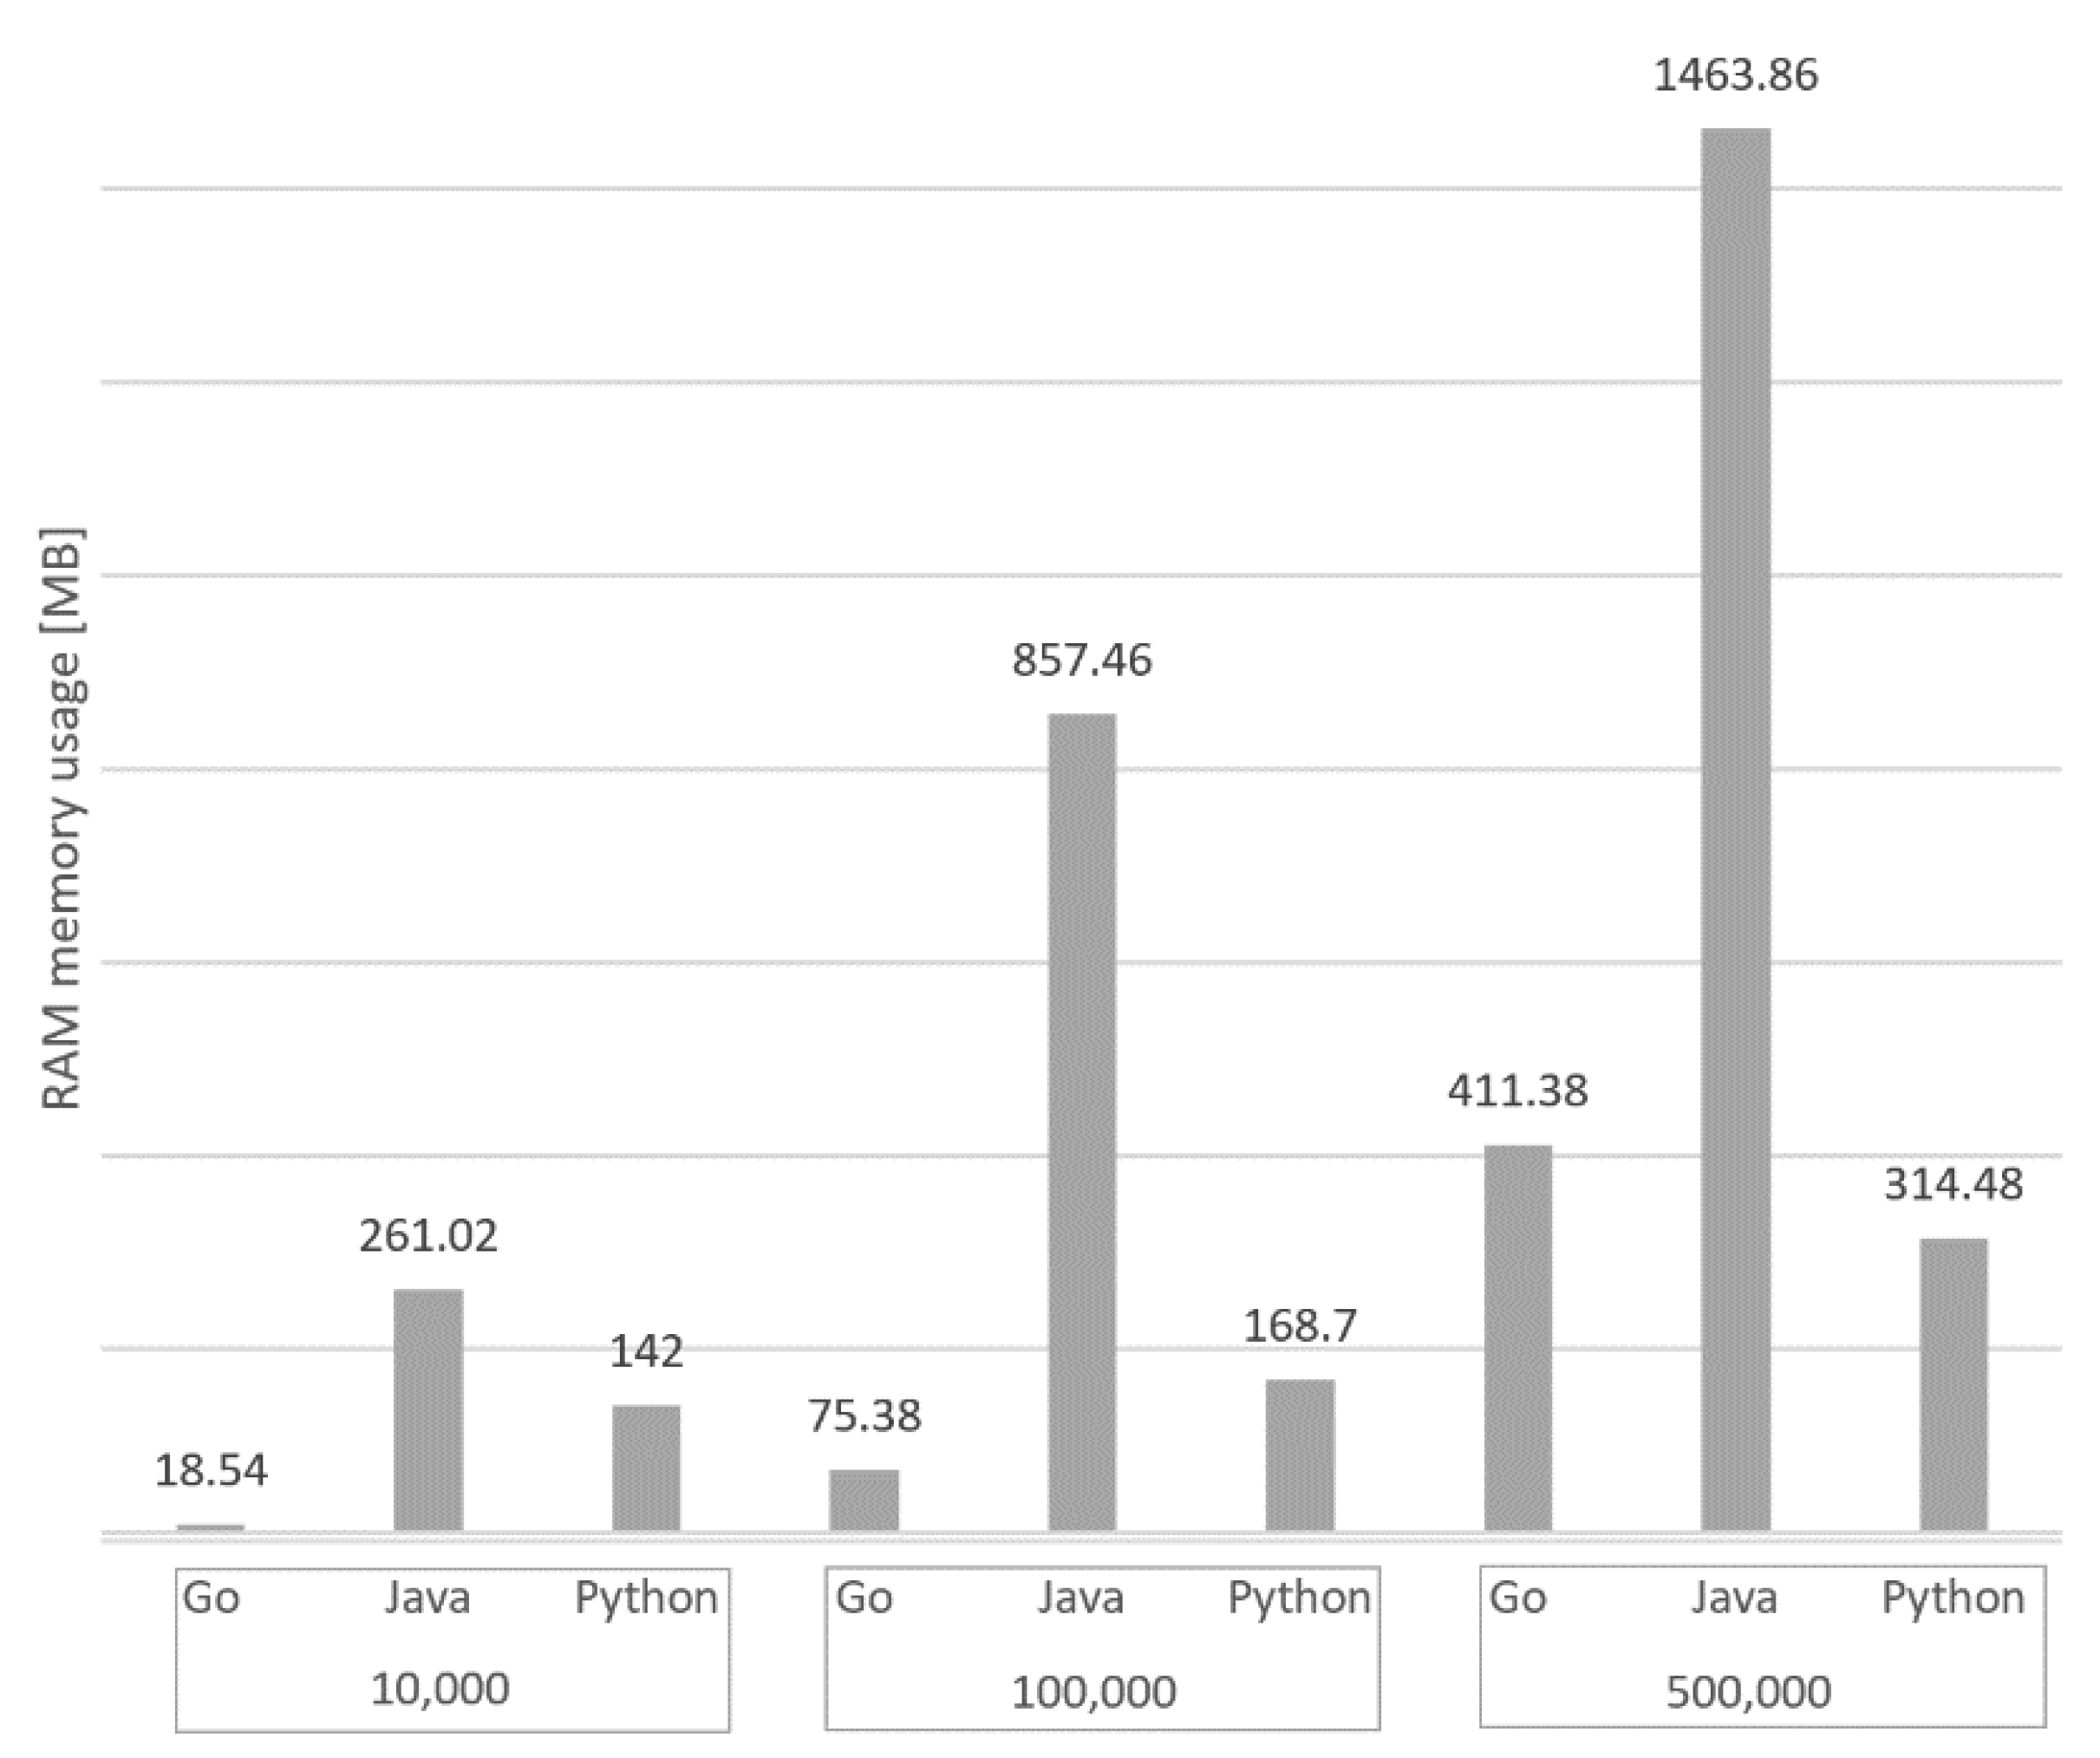
\includegraphics[height=0.3\textheight]{./part/Proyecto_ejecutivo/memoria_constructiva/golang/img/memory_usage}
	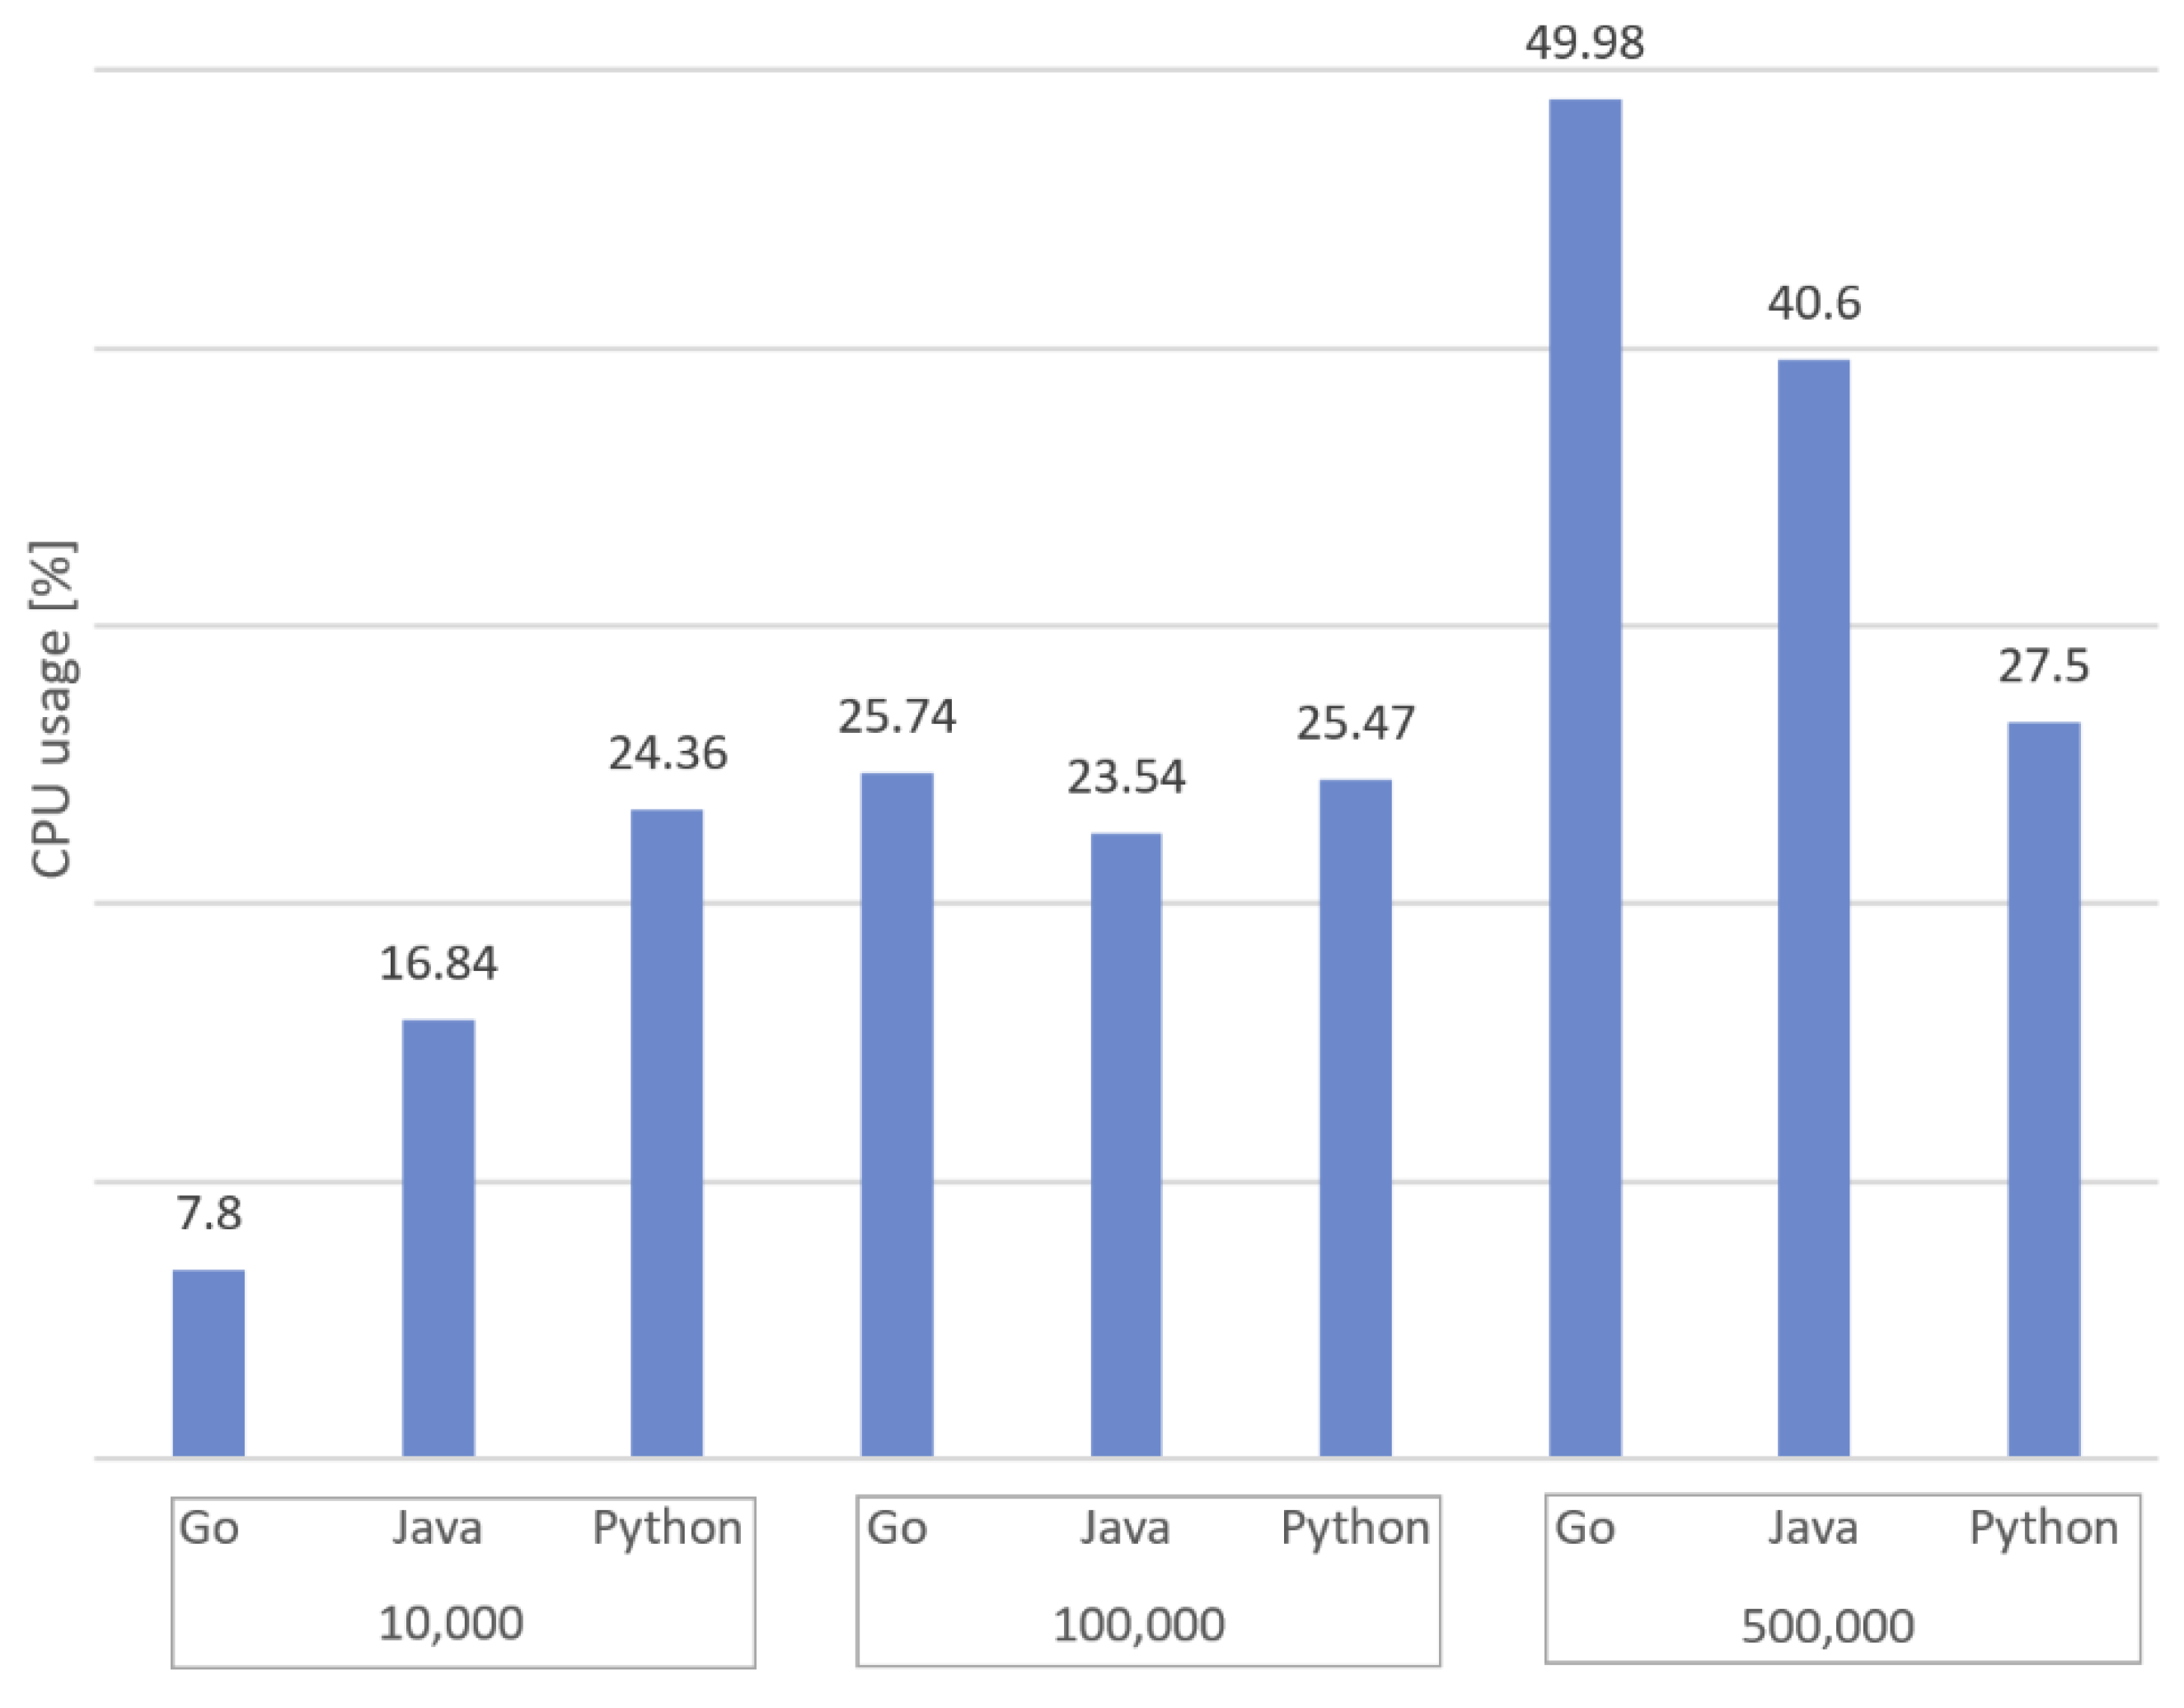
\includegraphics[height=0.3\textheight]{./part/Proyecto_ejecutivo/memoria_constructiva/golang/img/cpuUsage}
	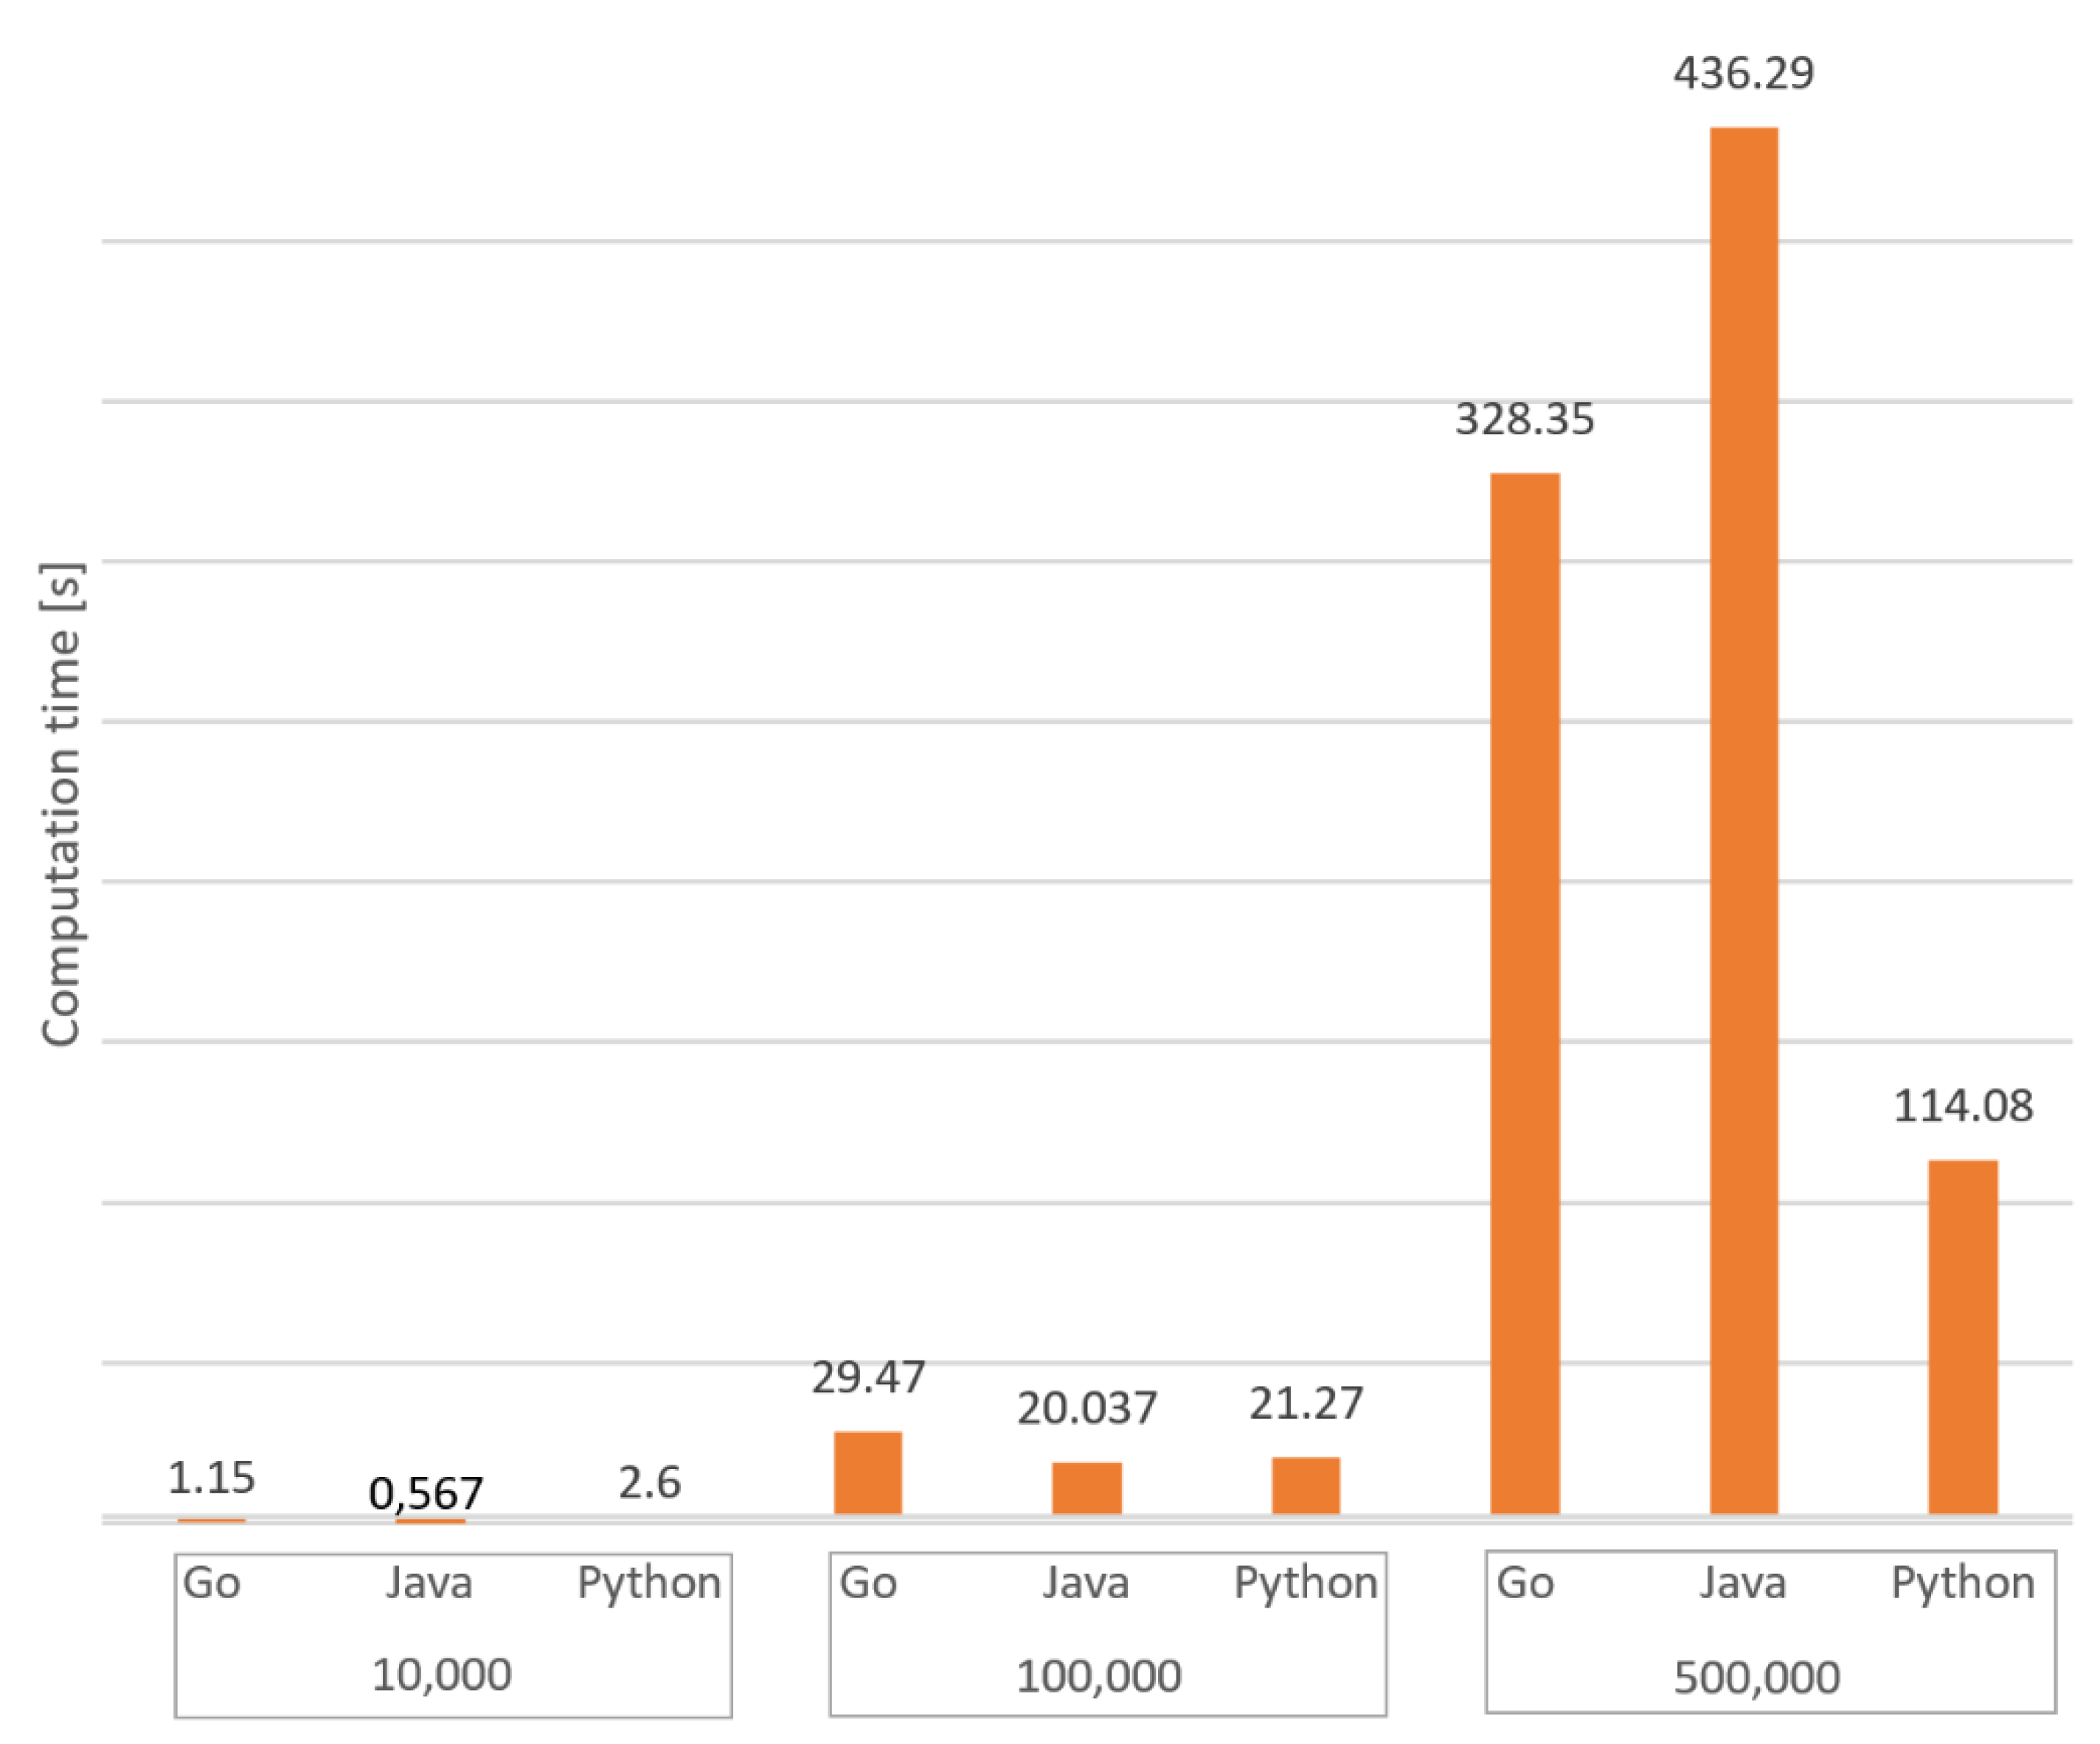
\includegraphics[height=0.3\textheight]{./part/Proyecto_ejecutivo/memoria_constructiva/golang/img/compTime}
	\caption[Estudio comparativo de rendimiento de Go, Python y Java]{performance golang on algorithm\cite{Dymora20201}}\label{fig:performance golang}
\end{figure}

La mejor virtud de Go como lenguaje viene de la mano de la facilidad de mantenimiento, la rapidez de compilación, el manejo fácil para la concurrencia y eficiente en el uso de recursos.
Implementar mecanismos de memoria compartida para procesos concurrente es donde golang optimiza recursos.
Uno cita de~\cite{Meyerson2014104+101}.
Trabajador de Google y contribuidor del ecosistema de Golang dice:
“Everyone knows and thinks about Google in terms of scale of users and scale of servers, but one thing that's not talked about as often is the scale of engineering effort.“.
Esto quiere decir que en la mayoría de las compañías el mayor coste no es el de infraestructura, si no el de ingeniería.
Es un factor más importante el reducir es el numero de horas dedicadas a mantener y desarrollar software que el hecho de optimizar el uso de máquinas.
Ante un problema que no requiera el uso intensivo de algorítmica o tiempo de respuesta en Go se encontraría la ventaja de reducir los recursos necesarios de infraestructura y los de ingeniería.
Si se diera el caso de que el software se enfrenta con el tiempo a problemas de escala siempre quedará la opción de aumentar las prestaciones de las máquinas utilizadas, pero evitaría tener problemas de aumento de costes de ingeniería.
El tiempo de compilación mientras se desarrolla un software puede llegar al orden de minutos por prueba en lenguajes como Java.
Este coste elevando al orden de magnitud de una empresa como Google puede significar una ingente cantidad de horas.

Las referencias consultas aplicados a distintos casos de uso extraen las mismas conclusiones acerca del nicho de uso de Golang y las bondades y puntos débiles del mismo:

\begin{itemize}
	\item uso para \textit{blockchain}~\cite{Ray202110857} o \textit{smart contracts}~\cite{Ding2021321},
	\item librerías para la depuración de códigos concurrentes~\cite{Taheri2021138},
	\item \textit{machine learning} para reconocimientos de lenguajes~\cite{NoAuthor2021179,Dilley2019377},
	\item uso para IoT ~\cite{Samaniego2017116},
	\item análisis de flujos de carga en sistemas eléctricos, haciendo uso de la concurrencia para resolver con mayor rapidez el cálculo~\cite{Khaitan20152909},
	\item y otros usos varios de la aplicación del paralelismo para la resolución de problemas~\cite{Qiu2018,Shoumik20181,Mladenovic2018,Benedict2017437,Irawan2017,Leokhin2015656,Komendantskaya2014121,Mittal2014292}.
\end{itemize}

Se extrae una cita más para presentar la conclusión final del estudio.
“Despite the relatively young age of the programming language, we believe that Go helps to fill an interesting niche in the field of programming languages.
The unique feature-set and aims of the language make it worth investigation for systems-level concurrent programming.“~\cite{WhiteheadII2011209}
Habiendo madurado el lenguaje unos años desde la publicación de este artículo sigue siendo relevante y está altamente valorado en la comunidad de desarrollo de software.
Permiten concluir que está justificado el objetivo de diseñar un sistema de las características de este proyecto con Go.

